
%***************************************************************************
%
% CreditCruncher - A portfolio credit risk valorator
% Copyright (C) 2004 Gerard Torrent
%
% This program is free software; you can redistribute it and/or
% modify it under the terms of the GNU General Public License
% as published by the Free Software Foundation; either version 2
% of the License.
%
% This program is distributed in the hope that it will be useful,
% but WITHOUT ANY WARRANTY; without even the implied warranty of
% MERCHANTABILITY or FITNESS FOR A PARTICULAR PURPOSE.  See the
% GNU General Public License for more details.
%
% You should have received a copy of the GNU General Public License
% along with this program; if not, write to the Free Software
% Foundation, Inc., 59 Temple Place - Suite 330, Boston, MA 02111-1307, USA.
%
%
% introduction.tex - TeX documentation file
% --------------------------------------------------------------------------
%
% 2004/12/04 - Gerard Torrent [gerard@fobos.generacio.com]
%   . initial release
%
%***************************************************************************

\chapter{Introduction to CreditCruncher}
\label{sec:introduction}

\section{About CreditCruncher}

CreditCruncher valora el riesgo de impago de una cartera de cr\'editos usando la 
t\'ecnica de simulaci\'on Monte Carlo. Es una implementaci\'on libre de la metodologia
CreditMetrics\footnote{http://www.riskmetrics.com/}. 

Se dispone de una cartera de N clientes donde cada cliente tiene contratado uno o 
varios productos con riesgo de cr\'edito. Cada cliente tiene asignado un rating de 
calidad crediticia y existe una matriz de transici\'on que permite determinar la 
probabilidad de fallido a un horizonte de tiempo fijado. Los clientes pertenecen 
a diversos sectores de los que disponemos de una matriz de correlaci\'on que 
indica el grado de dependencia intersectorial en caso de fallido. A partir de 
la matriz de correlaci\'on intersectorial se construye la matriz de correlaci\'on 
entre clientes. Finalmente se genera un conjunto de N variables aleatorias 
uniformes correlacionadas seg\'un esta matriz (c\'opula). Se usa la matriz de 
transici\'on para determinar la evoluci\'on del rating inicial de cada cliente y se 
evalua el valor de sus productos. Si se repite este proceso un n\'umero elevado de 
veces disponemos de un conjunto de valores posibles de la cartera que permiten 
determinar la distribuci\'on del valor de la cartera y calcular el VAR (Value At Risk). 
Para mas informaci\'on cons\'ultese el manual de CreditCruncher donde se describe 
con detalle todos los pasos realizados.

\begin{figure}[!hb]
\begin{center}
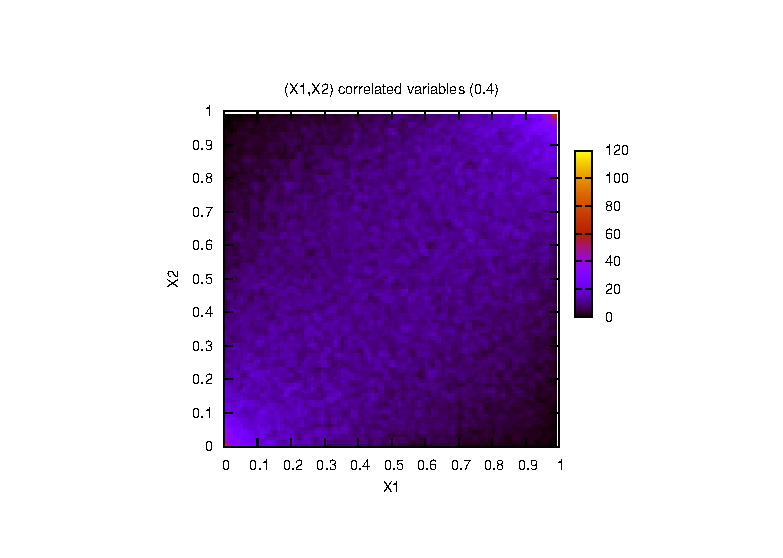
\includegraphics[height=5cm, angle=0]{./images/copula.eps}
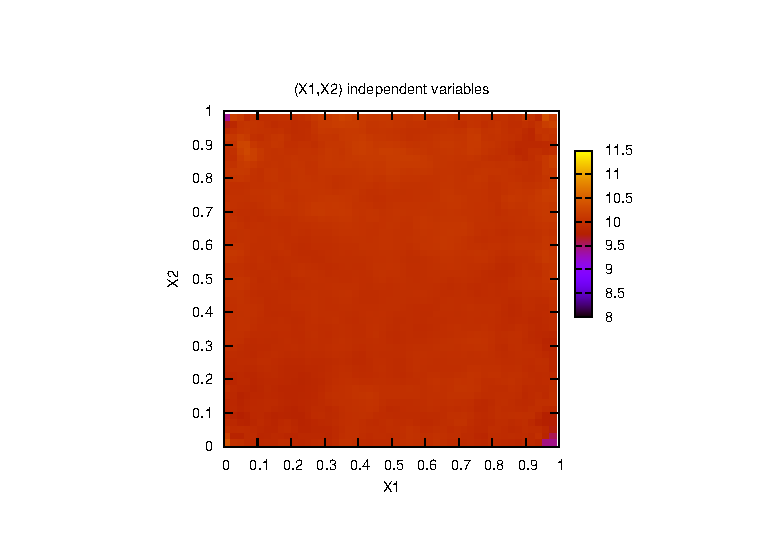
\includegraphics[height=5cm, angle=0]{./images/uniform.eps}
\caption{Bivariate distribution plot with correlation and independent}
\label{fig1}
\end{center}
\end{figure}

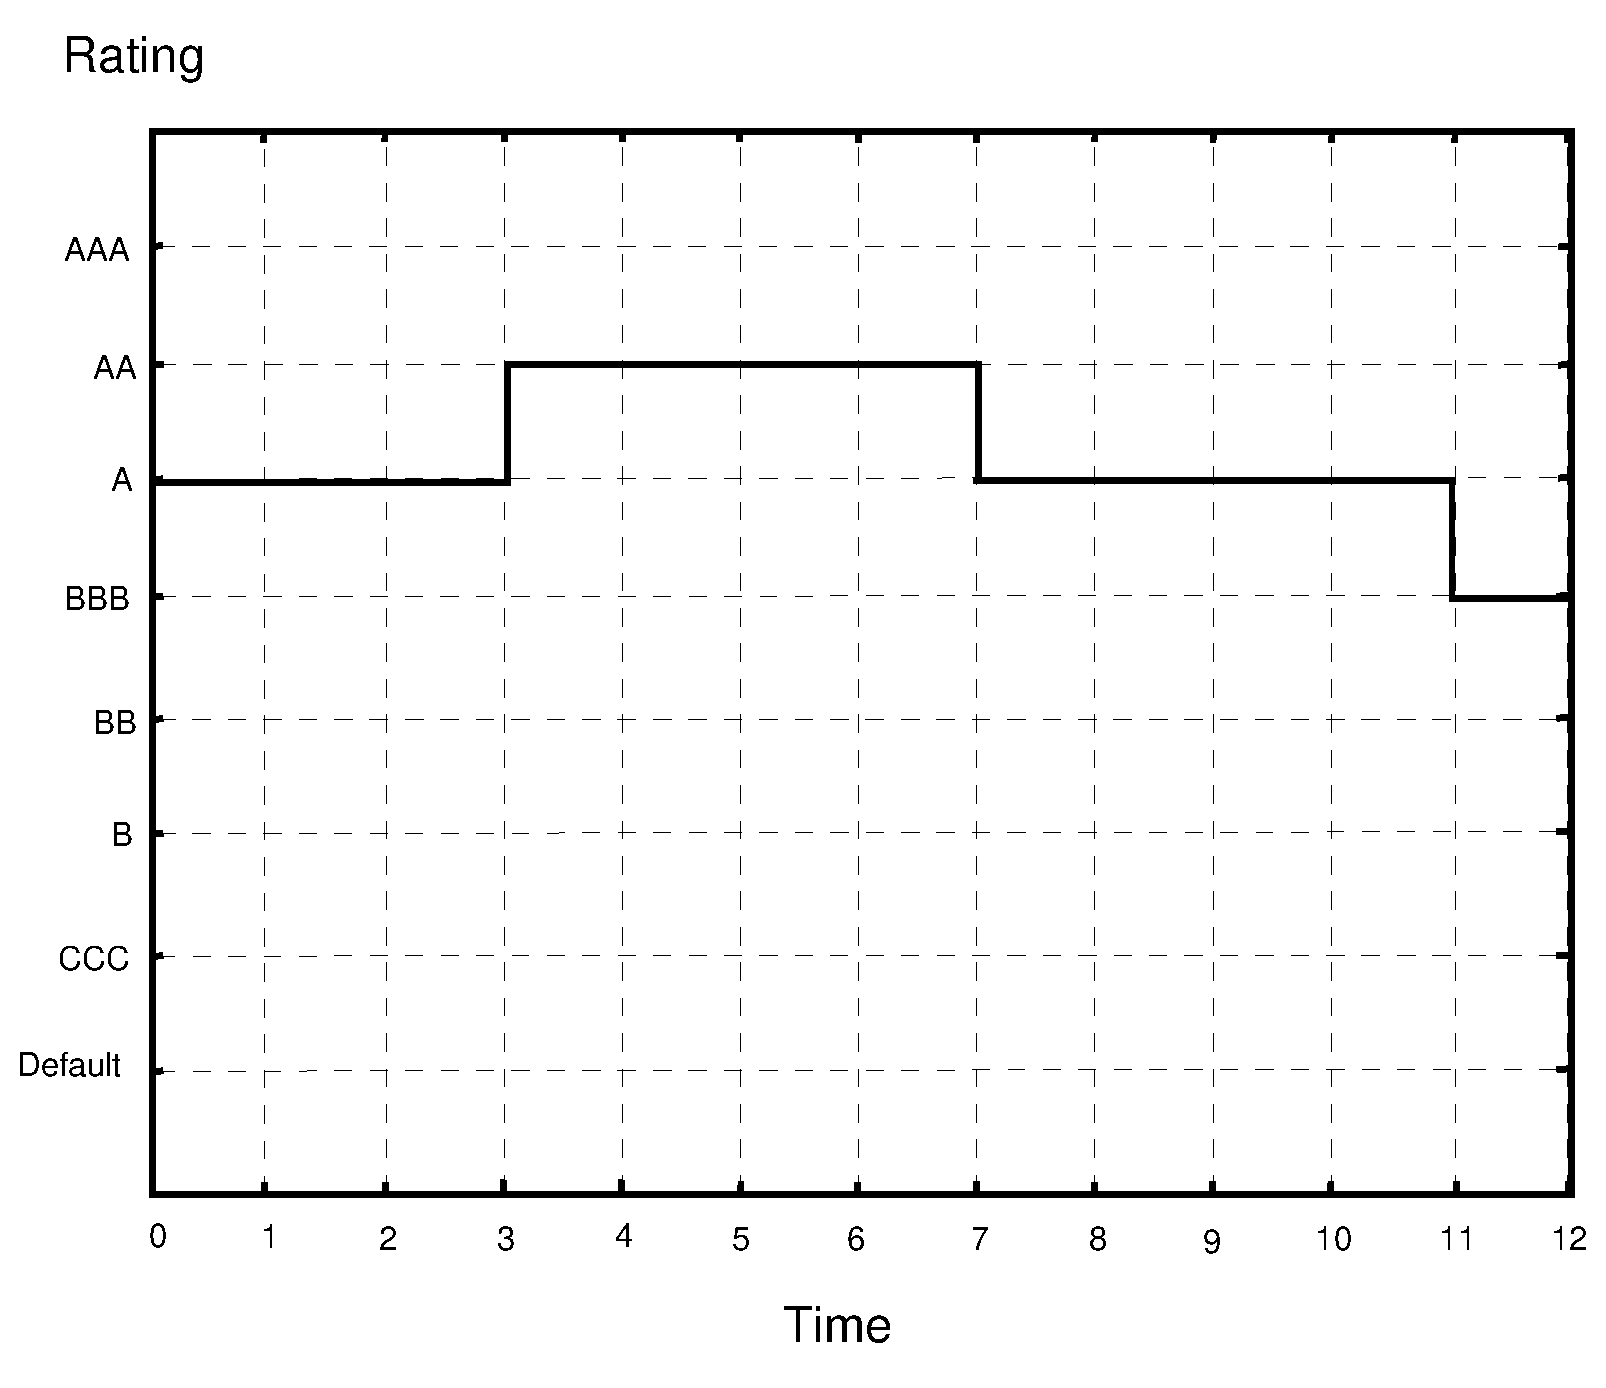
\includegraphics[height=7cm, angle=0]{./images/ratingevol.eps}

\chapter{Formulaci\'on del problema}
\label{sec:formulation}

\section{Hipotesis}

\paragraph{La \'unica fuente de riesgo es el riesgo de impago.}
No se contemplan los riesgos de variaci\'on de tipos de inter\'es, etc.

\paragraph{El tiempo est\'a repartido uniformemente.}
blablabla.

\paragraph{Un fallido no se recupera.}
blablabla.

\paragraph{Las probabilidades de fallido no dependen del tiempo.}
blablabla.

\paragraph{El rating y la recuperaci\'on de un cliente no depende de otro cliente.}
blablabla.


%===========================================================================

\section{La matriz de transici\'on}

\subsection{Definici\'on.} La matriz de transici\'on nos proporciona la probabilidad 
que un cliente con rating inicial $r_i$ pase a tener, al cabo de un tiempo $T$, 
rating $r_j$. La denotamos de la forma siguiente:

\begin{displaymath}
M_T = \left(
\begin{array}{ccc}
m_{1,1} & \dots  & m_{1,n} \cr
\vdots & \ddots & \vdots \cr
m_{n,1} & \dots  & m_{n,n} 
\end{array}
\right)
\end{displaymath}

\noindent donde cada elemento de la matrix, $m_{i,j}$ corresponde a la 
probabilidad de que un cliente con rating $r_i$ pase a tener, al cabo de $T$ 
tiempo, rating $r_j$.

\subsection{Ejemplo.} Matriz de transici\'on anual ($T=1$ año) extraida del 
documento \emph{CreditMetrics. Technical Document}. Las probabilidades est\'an
expresadas en tanto por ciento.
\\
\begin{center}
\begin{tabular}[]{l|rrrrrrrr}
        &      AAA &       AA &        A &      BBB &       BB &        B &      CCC &  Default \cr
\hline
AAA     &  $90.81$ &   $8.33$ &   $0.68$ &   $0.06$ &   $0.12$ &   $0.00$ &   $0.00$ &   $0.00$ \cr
 AA     &   $0.70$ &  $90.65$ &   $7.79$ &   $0.64$ &   $0.06$ &   $0.14$ &   $0.02$ &   $0.00$ \cr
  A     &   $0.09$ &   $2.27$ &  $91.05$ &   $5.52$ &   $0.74$ &   $0.26$ &   $0.01$ &   $0.06$ \cr
BBB     &   $0.02$ &   $0.33$ &   $5.95$ &  $86.93$ &   $5.30$ &   $1.17$ &   $0.12$ &   $0.18$ \cr
 BB     &   $0.03$ &   $0.14$ &   $0.67$ &   $7.73$ &  $80.53$ &   $8.84$ &   $1.00$ &   $1.06$ \cr
  B     &   $0.00$ &   $0.11$ &   $0.24$ &   $0.43$ &   $6.48$ &  $83.46$ &   $4.07$ &   $5.20$ \cr
CCC     &   $0.22$ &   $0.00$ &   $0.22$ &   $1.30$ &   $2.38$ &  $11.24$ &  $64.86$ &  $19.79$ \cr
Default &   $0.00$ &   $0.00$ &   $0.00$ &   $0.00$ &   $0.00$ &   $0.00$ &   $0.00$ & $100.00$
\end{tabular}
\end{center}
\noindent en particular, la probabilidad que un cliente con rating $AA$ pase a 
tener rating $B$ al cabo de un año es del $0.14\%$.

\subsection{Propiedades}

\paragraph{Propiedad 1.}
El valor de los elementos de la matriz de transici\'on se encuentran entre $0$ 
y $1$ debido a que son probabilidades.

\begin{displaymath}
0 \leq m_{i,j} \leq 1 \quad \forall i,j
\end{displaymath}

\paragraph{Propiedad 2.}
La suma de los elementos de cualquier fila de la matriz de transici\'on suman $1$.
De esta forma se  est\'a imponiendo que el conjunto de ratings finales solo puede 
ser el de los ratings contemplados en la matriz.

\begin{displaymath}
\sum_{j=1}^{n} m_{i,j} = 1 \quad \forall i
\end{displaymath}

\paragraph{Propiedad 3.}
Los elementos de la fila correspondiente al rating $default$, son todos $0$,
excepto el elemento de la columna que corresponde al rating $default$ que vale 
$1$. Esta condici\'on indica que cuando se llega al estado de fallido no es 
posible salir de este estado.

\begin{displaymath}
\begin{array}{ll}
m_{default,j} = 0        & \quad \forall j \neq default \cr
m_{default,default} = 1
\end{array}
\end{displaymath}


\subsection{Cambio de periodo}

Deseamos obtener la matriz de transici\'on para periodos distintos (m\'ultiplos o 
fraccionarios) del periodo proporcionado, $T$. Esto nos permitir\'a determinar la 
probabilidad que un cliente con rating inicial $r_i$ tenga rating $r_j$ al cabo 
de $x \cdot T$ tiempo.

\paragraph{Ejemplo.} Calculemos la probabilidad de pasar de rating $AA$ a
rating $B$ en un plazo de dos años disponiendo de la matriz de transici\'on anual.

\begin{displaymath}
\begin{array}{llll}
P(AA \to B;2) = & P(AA \to AAA;1)    & \cdot P(AAA \to B;1)      & + \cr
                & P(AA \to AA;1)      & \cdot P(AA \to B;1)      & + \cr
                & P(AA \to A;1)       & \cdot P(A \to B;1)       & + \cr
                & P(AA \to BBB;1)     & \cdot P(BBB \to B;1)     & + \cr
                & P(AA \to BB;1)      & \cdot P(BB \to B;1)      & + \cr
                & P(AA \to B;1)       & \cdot P(B \to B;1)       & + \cr
                & P(AA \to CCC;1)     & \cdot P(CCC \to B;1)     & + \cr
                & P(AA \to default;1) & \cdot P(default \to B;1) &
\end{array}
\end{displaymath}

\paragraph{Proposici\'on} Sean $M_{T_1}$ y $M_{T_2}$ las matrices de transici\'on
para los periodos $T_1$ y $T_2$. Entonces, la matriz de transici\'on para el
periodo $T_1+T_2$ es:
\begin{displaymath}
M_{T_1+T_2} = M_{T_1} \cdot M_{T_2}
\end{displaymath}

\paragraph{Corolario} Sean $M_{T}$ la matriz de transici\'on para el periodo 
$T$ y $k \in \mathrm{N}$. Entonces:
\begin{displaymath}
M_{k \cdot T} = M_{T}^k
\end{displaymath}
\begin{displaymath}
M_{\frac{T}{k}} = \sqrt[k]{M_{T}}
\end{displaymath}


%===========================================================================

\section{C\'alculo de la raiz de una matriz}

\paragraph{Definici\'on.}
Diremos que 2 matrices $A$ y $B$ de orden $n$ son semejantes si existe una 
matriz, $P$, de orden $n$ con $det(P) \neq 0$ tal que 
$B = P^{-1} \cdot A \cdot P$.


\paragraph{Proposici\'on.} Si dos matrices $A$ y $B$ son semejantes 
($B = P^{-1} \cdot A \cdot P$) entonces:
\begin{displaymath}
det(A) = det(B)
\end{displaymath}
\begin{displaymath}
B^n = P^{-1} \cdot A^{n} \cdot P
\end{displaymath}

\paragraph{Definici\'on.} 
Diremos que Una matriz $A$ de orden $n$ es diagonalizable si es semejante a una 
matriz diagonal $D$, o sea, $A = P^{-1} \cdot D \cdot P$ siendo $det(D) \neq 0$.

\paragraph{Proposici\'on.} 
Para que una matriz $A$ sea diagonalizable es necesario y suficiente que:
\begin{itemize}
\item Los valores propios de $A$ sean todos reales
\item Los $n$ vectores propios de $A$ sean independientes
\end{itemize}

\paragraph{Proposici\'on.}
Si una matriz $A$ es diagonalizable ($A = P^{-1} \cdot D \cdot P$) entonces: 
\begin{itemize}
\item $D$ es una matriz diagonal compuesta por los valores propios de la matriz $A$
\item $P$ es la matriz formada por los vectores propios de la matriz $A$
\end{itemize}

\paragraph{Resultado.}
Sea $A$ la ra\'iz $n$-esima de una matriz diagonalizable $B$. Entonces:
\begin{displaymath}
A^n = B = P^{-1} \cdot D \cdot P 
\Longrightarrow  
A = \sqrt[n]{B} = P^{-1} \cdot \sqrt[n]{D} \cdot P
\end{displaymath} 


%===========================================================================

\section{La variable aleatoria normal}

\subsection{Definici\'on y propiedades}

\begin{displaymath}
P(X \leq x) = \Phi(x) = \int_{-\infty}^{x} \frac{e^{-t^2}}{\sqrt{2 \pi}} dt
\end{displaymath}

\subsection{Simulaci\'on}

Para la generaci\'on de una realizaci\'on, $z$, de una variable aleatoria normal  
$Z \sim N(\mu, \sigma)$ utilizamos el siguiente algoritmo:

\begin{displaymath}
z = \mu + \sigma\cdot \sqrt{-2 \cdot ln(u[0,1])} \cdot cos(2 \cdot \pi \cdot u[0,1])
\end{displaymath}

\noindent donde $u[0,1]$ son realizaciones de una variable aleatoria uniforme 
en el intervalo $[0,1]$.

%===========================================================================

\section{Copulas. Variables aleatorias correlacionadas}

\paragraph{Definici\'on.}
Una copula es la funci\'on de distribuci\'on de un vector aleatorio sobre 
$\Re^n$ donde las funciones de distribuci\'on marginales son $U[0,1]$. 
\begin{displaymath}
C(u_1, \cdots, u_n) = P\{U_1 \leq u_1, \cdots, U_n \leq u_n\}
\end{displaymath}

\paragraph{Proposici\'on.}
$C$ es una c\'opula $\iff C:[0,1]^n \to [0,1]$ y cumple las siguientes 
propiedades:
\begin{itemize}
\item $C(x_1, \cdots, x_n)$ es creciente en cada componente $x_i$
\item $C(1, \cdots, 1, x_i, 1, \cdots, 1) = x_i \quad \forall i \in \{1, \cdots, n\}, x_i \in [0,1]$
\item $\forall (a_1, \cdots, a_n) \in [0,1]^n$ y $\forall (b_1, \cdots, b_n) \in [0,1]^n$ con
$a_i \leq b_i$ se cumple:
\begin{displaymath}
\sum_{i_1=1}^{2} \cdots \sum_{i_n=1}^{2} (-1)^{i_1+\cdots+x_n} C(x_{1i_1},\cdots,x_{ni_n}) \geq 0
\end{displaymath}
\noindent siendo $x_{j1}=a_j$ y $x_{j2}=b_j$ $\quad \forall j \in \{1, \cdots, n\}$
\end{itemize}

\paragraph{Generaci\'on de c\'opulas normales o arquimedianas.}

Sea $(Z_1,\cdots, Z_n)$ un vector aleatorio con marginales $Z_i \sim N(0,1)$ con
\begin{displaymath}
\Sigma = \left( 
\begin{array}{cccc}
1          & \rho_{12} & \ldots & \rho_{1n} \cr
\rho_{21} & 1          & \ldots & \rho_{2n} \cr
\vdots    & \vdots    & \ddots & \vdots   \cr
\rho_{n1} & \rho_{n2} & \ldots & 1
\end{array}
\right)
\end{displaymath}

\noindent siendo $\rho_{ij} = \rho_{ji}$ el coeficiente de correlaci\'on entre 
$Z_i$ y $Z_j$.

\noindent Calculamos la raiz de $\Sigma$ usando el algoritmo de Cholesky. 
De esta forma obtenemos la matriz triengular inferior
\begin{displaymath}
B = 
\left(
\begin{array}{cccc}
b_{11}   & 0        & \ldots & 0       \cr
b_{21}   & b_{22}   & \ldots & 0       \cr
\vdots  & \vdots  & \ddots & \vdots \cr
b_{n1}   & b_{n2}   & \ldots & b_{nn}
\end{array}
\right)
\end{displaymath}

\noindent que cumple $B \cdot B' = \Sigma$

\noindent Generamos una simulaci\'on del vector aleatorio $Y=(Y_1, \cdots, Y_n)'$ 
donde $Y_k \sim N(0,1)$ son variables aleatorias independientes.

\noindent Calculamos $Z = B \cdot Y$. El vector aleatorio resultante, $Z$ tiene
marginales $Z_k \sim N(0,1)$ y se encuentran correlacionadas seg\'un la matriz 
$\Sigma$.

\noindent Calculamos $X = (X_1, \cdots, X_n)'$ de la forma:
\begin{displaymath}
x_i = \Phi^{-1}(y_i)
\end{displaymath}

\noindent donde $\Phi(x) = \int_{-\infty}^{x} \frac{1}{\sqrt{2 \pi}} e^{-t^2} dt$
